	\makeatother
%	\author{Mitesh M. Khapra}
	\title{Module 4}
	\subtitle{Cats}
		\author{}
		\institute{}
	\date{}
%\institute{Department of Computer Science and Engineering\\ Indian Institute of Technology Madras}
%\titlegraphic{
\includegraphics[height=1cm,width=2cm]{images/iitm_logo.png}}
%\titlegraphicii{\includegraphics[height=1cm,width=2cm]{logo2}}

\begin{frame}
	\myheading{Chapter 4: Cats}
\end{frame}

\begin{frame}
\begin{minipage}[t][0.6\textheight][t]{\textwidth}
\begin{columns}
\column{0.5\textwidth}
\begin{overlayarea}{\textwidth}{\textheight}
\justify
\only<1>{\myheading{Hubel and Wiesel Experiment} Experimentally showed that each neuron has a fixed receptive field - i.e. a neuron will fire only in response to a visual stimuli in a specific region in the visual space \cite{wiesel:1959}}
\only<2>{\myheading{Neocognitron} Used for Handwritten character recognition and pattern recognition (Fukushima et. al.) \cite{fukushima:1980}}
\only<3>{\myheading{Convolutional Neural Network} Handwriting digit recognition using backpropagation over a Convolutional Neural Network (LeCun et. al.) \cite{LeCun:89}}
\only<4>{\myheading{LeNet-5} Introduced the (now famous) MNIST dataset (LeCun et. al.)\cite{LeCun:98}}
\end{overlayarea}
\column{0.5\textwidth}
\begin{overlayarea}{\textwidth}{\textheight}
\begin{figure}
\centering
\only<1>{\includegraphics[scale=0.3]{"images/Renewed_Interest/CNN_History/1959"}}
\only<2>{\includegraphics[scale=0.5]{"images/Renewed_Interest/CNN_History/1980"}}
\only<3>{\includegraphics[scale=0.5]{"images/Renewed_Interest/CNN_History/1989"}}
\only<4>{\includegraphics[scale=0.5]{"images/Renewed_Interest/CNN_History/1998"}}
\end{figure}
\end{overlayarea}
\end{columns}
\end{minipage}
\begin{minipage}[t][0.4\textheight][t]{\textwidth}
\begin{overlayarea}{\textwidth}{\textheight}
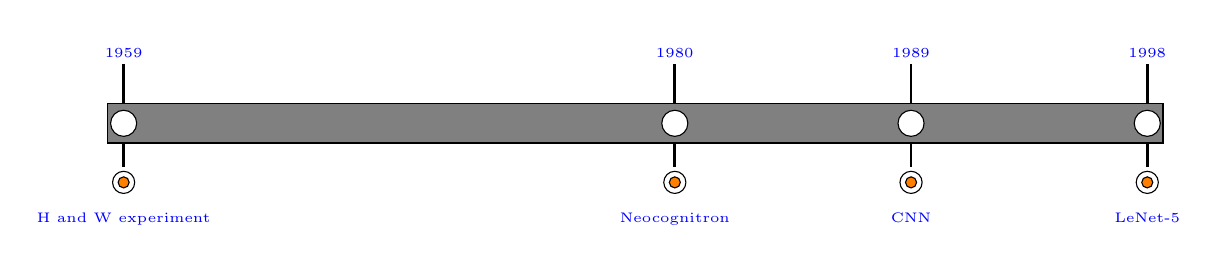
\begin{tikzpicture}[datemarker/.style={circle, draw=black,fill=white},textlabel/.style={anchor=center,text height=1.7ex,text depth=.25ex}] 
\tikzset{every node/.style={font=\tiny, color=blue}}\draw[fill=gray](-0.2,0) rectangle (13.2,0.5) node[white, below]{}; 
\onslide<1->{\node at (0.0, 0.25) [datemarker] {};}
\onslide<1->{\draw [line width=1pt] (0.0, 0.5) to (0.0, 1.0);} 
\onslide<1->{\draw (0.0, 1.2) node [textlabel] {1959 };}
\onslide<1->{\draw [fill=orange](0.0, -0.5) circle (2pt){};}
\onslide<1->{\draw (0.0, -0.5) circle (4pt){};}
\onslide<1->{\draw [line width=1pt] (0.0, 0) to (0.0, -0.3);}
\onslide<1->{\draw (0.0,-0.9) node [textlabel] {H and W experiment};}

\onslide<2->{\node at (7.0, 0.25) [datemarker] {};}
\onslide<2->{\draw [line width=1pt] (7.0, 0.5) to (7.0, 1.0);} 
\onslide<2->{\draw (7.0, 1.2) node [textlabel] {1980 };}
\onslide<2->{\draw [fill=orange](7.0, -0.5) circle (2pt){};}
\onslide<2->{\draw (7.0, -0.5) circle (4pt){};}
\onslide<2->{\draw [line width=1pt] (7.0, 0) to (7.0, -0.3);}
\onslide<2->{\draw (7.0,-0.9) node [textlabel] {Neocognitron};}

\onslide<3->{\node at (10.0, 0.25) [datemarker] {};}
\onslide<3->{\draw [line width=1pt] (10.0, 0.5) to (10.0, 1.0);} 
\onslide<3->{\draw (10.0, 1.2) node [textlabel] {1989 };}
\onslide<3->{\draw [fill=orange](10.0, -0.5) circle (2pt){};}
\onslide<3->{\draw (10.0, -0.5) circle (4pt){};}
\onslide<3->{\draw [line width=1pt] (10.0, 0) to (10.0, -0.3);}
\onslide<3->{\draw (10.0,-0.9) node [textlabel] {CNN};}

\onslide<4->{\node at (13.0, 0.25) [datemarker] {};}
\onslide<4->{\draw [line width=1pt] (13.0, 0.5) to (13.0, 1.0);} 
\onslide<4->{\draw (13.0, 1.2) node [textlabel] {1998 };}
\onslide<4->{\draw [fill=orange](13.0, -0.5) circle (2pt){};}
\onslide<4->{\draw (13.0, -0.5) circle (4pt){};}
\onslide<4->{\draw [line width=1pt] (13.0, 0) to (13.0, -0.3);}
\onslide<4->{\draw (13.0,-0.9) node [textlabel] {LeNet-5};}
\end{tikzpicture}
\end{overlayarea}
\end{minipage}
\end{frame}

\begin{frame}
    \myheading{An algorithm inspired by an experiment on cats is today used to detect cats in videos :-)}
\end{frame}